\chapter{Implementation}
\label{ch:Implementation}
\begin{figure}
	\centering
	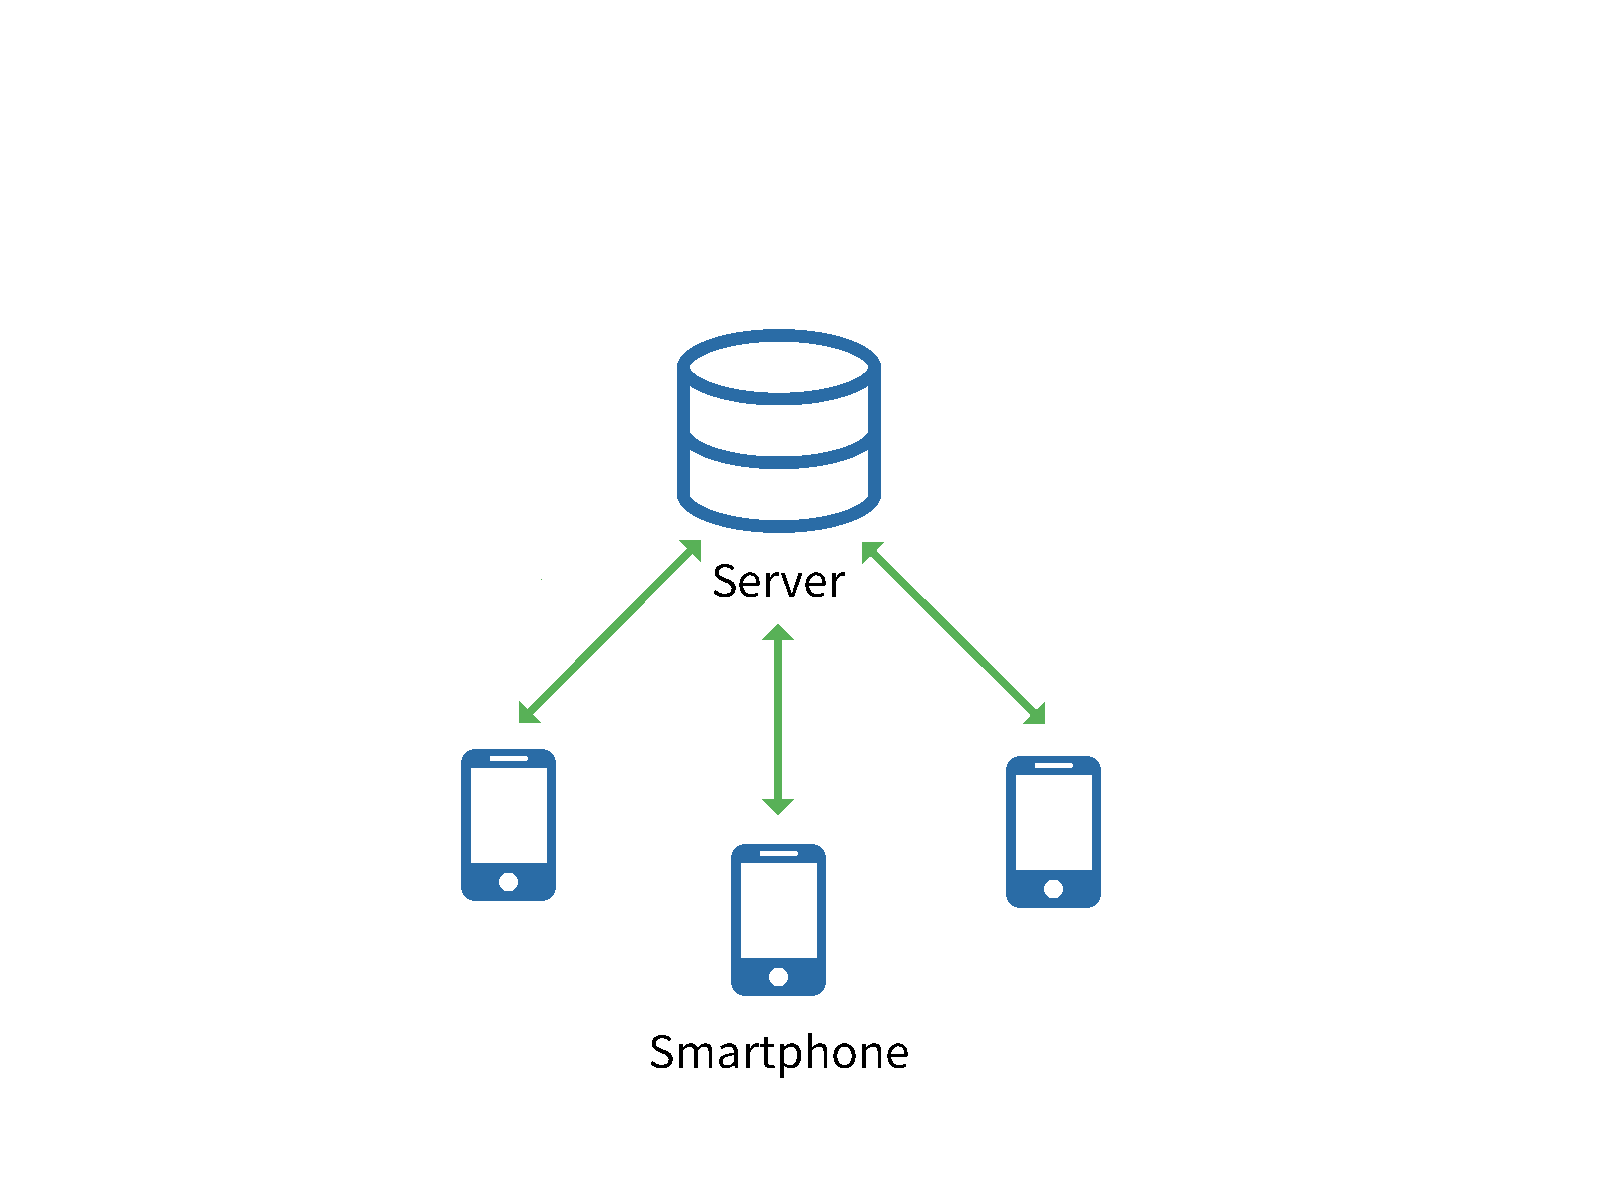
\includegraphics[height=6cm]{logos/client-server.png}
	\caption{Our client-server model}
	\label{img:client-server}
\end{figure}
The system is implemented according to the client-server model (figure \ref{img:client-server}). Users utilize a smartphone as a client, while the operator provides a server on which a central database is hosted. Also running on the server is a web service that can be requested by the clients via a REST API. The web service forwards the request to the database system and also returns the response back to the clients. An Android prototype was developed for the clients using Java. The web service is also written in Java and runs on a Tomcat server, while a MySQL server has been set up for the database system. In total, the implementation consists of three relatively independent parts, which will be examined in more detail below. The final realization of the $SPS$ is of course not part of this work or the implementation, but the last part of this section should give some comments on a possible realization. These include, for example, how to deal with the problem described at the end of section \ref{sec:Adversary Model and Assumptions} of adversaries not registered in the system.

\begin{figure}
	\centering
	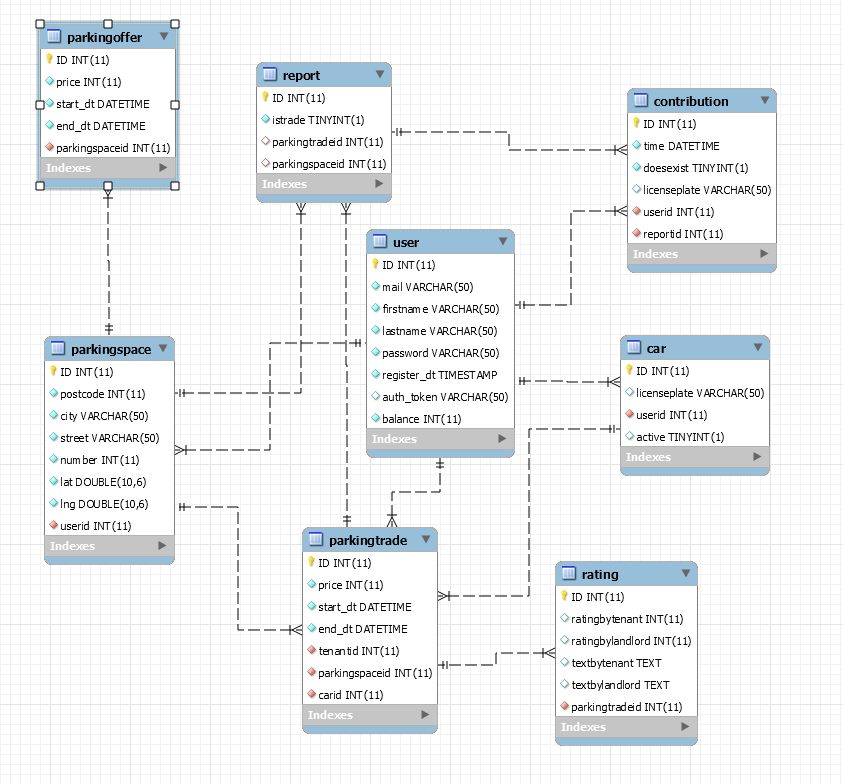
\includegraphics[width=14cm]{logos/eer-diagramm.png}
	\caption{The EER Diagramm of the database}
	\label{img:eer-diagramm}
\end{figure}

\section{Database}
A relational database management system was used to store user and parking data. We chose the open source system MySQL, which, as the name suggests, uses SQL as the query language. The actual database system, whose EER diagram is depicted in figure \ref{img:eer-diagramm}, consists of the following tables:
\begin{itemize}
\item \textbf{user:} Table \textit{user} represents a user $u \in U$ and stores attributes like mail, name, encrypted password, balance or reputation score.
\item \textbf{parkingspace:} Table \textit{parkingspace} represents a parking space $p \in P$ registered by a user and stores attributes like the address, coordinates and references the \textit{user}, who registered the parking space, with a foreign key constraint.
\item \textbf{parkingoffer:} Table \textit{parkingoffer} represents a parking offer created by a user for one of his parking spaces and stores attributes like offer starting time, offer ending time, price per hour and references the \textit{parkingspace}, for which the  offer was created for, with a foreign key constraint and thus allows to also figure out the user that created it.
\item \textbf{car:} Table \textit{car} represents a car registered by a user and stores the license plate, whether or not it is the active car of the user and references the \textit{user}, who registered the car, with a foreign key constraint. Every user can have a maximum of one car active at a time. If a user books a parking space this car is referenced in the \textit{parkingtrade} table.
\item \textbf{parkingtrade:} Table \textit{parkingtrade} represents a parking trade or contract between two users and stores attributes like booked starting time, booked ending time, price per hour and references the tenant \textit{user} and his \textit{car} as well as the \textit{parkingspace}, that was booked, with foreign key constraints and thus allows to also figure out the landlord that owns the parking space.
\item \textbf{rating:} Table \textit{rating} represents a rating for a parking trade and stores the rating value and text by both the landlord and the tenant of the parking trade and references the \textit{parkingtrade}, for which this rating was issued, with a foreign key constraint.
\item \textbf{report:} Table \textit{report} represents a report for a parking trade or parking space and stores for which one of the two the report is issued and references the \textit{parkingtrade} or \textit{parkingspace}, for which this report is issued, and the reported and reporting \textit{user}s with foreign key constraints.
\item \textbf{contribution:} Table \textit{contribution} represents a contribution to a report and stores the inspection time, whether the reported parking place exists, the license plate of the car parked on it at inspection time and references the \textit{user}, who gave the contribution, and the \textit{report}, for which this contribution applies, with foreign key constraints.
\end{itemize}

\subparagraph{Instructions for use}
To avoid having to recreate the database, a dump \textit{shared\_parking\_dump.sql} has been created that can be used to restore the database. This back up is located on the attached CD in the directory 'database'.

\section{Java Web Service}
A web service in Java was developed to access the database. It runs on a Tomcat server and offers a RESTful interface. This interface is used by the android app to access the database. The java open source framework Jersey is used to develop the REST API. This framework helps to address JAX-RS, the Java API for RESTful Web Service. For this purpose, annotations are used in the code that can be found in the java package javax.ws.rs. These annotations are used to specify the path and the request method, which are both part of an http request, by which a java method may be addressed.\\

The java code for the web service can be found on the attached CD in the directory 'web\_service'. The .java classes can be found in \textit{shared\_parking/src/com/shared\_parking}.

The package \textit{jersey} contains classes for every database table, in which the already addressed annotations are used to tell jersey for which HTTP request to listen. In these classes the web service functions are described. Those get called when the Tomcat server receives an appropriate HTTP request. For most of the tables the basic functions of persistent storage \textit{create, read, update and delete (CRUD)} are implemented. For some tables there are multiple \textit{read} functions, depending on how they are required by the android prototype. Car.java for example has two read methods: one for reading all cars by a user, another one for reading only the active car by a user. The data transferred between these web service functions and the android app is always in the form of JSON objects. Each of those functions receives their parameters as a JSON object in the body of the HTTP request and returns the result as a JSON object in the body of the HTTP response. The JAX-RS annotations used for all of our functions tell those function to listen to HTPP POST requests with MediaType.APPLICATION\_JSON as input and return value. After receiving a request, these web service functions then deconstruct the JSON Object into the represented parameters and calls another method, which then accesses the database.

The methods used for Database access can be found in the package \textit{dbconnection}. There is a database connection method for every web service function. The database connection methods take the deconstructed JSON object as parameters. They then open a database connection with the help of the java.sql package and create and execute the appropriate SQL querys. After receiving the Resultset from the database they call a utility method to create a JSONObject as the result and return it to the web service methods, which they then put into the HTTP response.

The utility methods can be found in the \textit{utility} package. They accept a java.sql Resultset and construct a JSON object from it, which they then return back to the database connection methods. 

\subparagraph{Instructions for use}
There is a class called Constants.java in the \textit{dbconntection} package. In there one has to change the parameters for database access, so that they match with the access information of ones own database. The whole project can for example be imported into Eclipse and the web service methods can be run in there on a Tomcat server.

\section{Java Android Prototype}
The main part of the implementation was the development of the android app, which is also written with java. The app uses Gradle as a build automation system. The development of the UI largely adheres to the guidelines set by Google regarding material design. This ensures that new users can find their way around the app in no time. The app itself has no internal database and mainly uses JSON objects to manage the user and parking data, since the data is returned in this form by the Web service. These objects are only stored in the random access memory and the corresponding web service is queried again if necessary.

For remembering a user session an auth\_token is stored in the Android Shared Preferences. This prevents the user from having to constantly enter his password. Despite that, the other information security features mentioned in the beginning of section \ref{Security Requirements}, like the encrypted network traffic, are not implemented as this is still a prototype used for testing.

The prototype implements all functional design features. Instead of giving the user the ability to charge and withdraw money, buttons are added which allow to adjust the balance of a user. Of the security design features, only the report module is implemented in the prototype. The other features are not necessary for an initial function test and only become meaningful when a test run is started with several users.

The java code for the prototype can be found on the attached CD in the directory 'android'. All the Gradle files can be directly found in this directory and in the subdirectories '.gradle' and 'gradle'. The .java classes can be found in \textit{app\-/main\-/ja\-va\-/com\-/e\-xam\-ple\-/sha\-red\-\_par\-king\-/src\-/com\-/sha\-red\-\_par\-king}. The .xml layout and menu files and the icons used for the UI can be found in \textit{app/main/res} in the corresponding subdirectories. The .java classes are divided into the package \textit{activities}, which contains all the code for the android activities and fragments and the package \textit{networking}, which contains all the code needed for getting access to the database through the web service functions by sending HTTP requests.

The class NetworkUtilities.java in the \textit{networking} package contains a static method for every CRUD web service function available. Those methods first construct the JSON object added into the body of the http request and then use the HTTP library Volley to send a HTTP request. The JSON object that is returned by the web service can processed through the implementation of a callback interface called ServerCallback.java.

The \textit{activities} package is further divided. First, there is the BaseActivity.java which defines the Toolbar and the DrawerLayout with integrated NavigationView. Every other activity class extends this BaseActivity, thus enabling the toolbar and the drawer menu at all times. Each menu item in this drawer menu (figure \ref{img:screenshot-menu}) has its own subpackage containing the corresponding activity and all corresponding fragments. The following menu items and packages exist:

\begin{itemize}
\item \textbf{Home:} The java classes for the 'Home' menu item are found in the \textit{main} package. The package contains the MainActivity and two fragments, which provide the ability for the user to log in and register.
\item \textbf{Search for parking:} The java classes for the 'Search for parking' menu item are found in the \textit{search} package. The package contains the SearchActivity, which displays a SupportMapFragment, and two DialogFragments. The SupportMapFragment shows a map provided by Google, on which the available parking spaces are displayed as markers (figure \ref{img:screenshot-search}). The DialogFragments serve on the one hand to select the date and time at which a parking space should be searched for (TimeDialogFragment), on the other hand to display information about this parking space with the possibility of confirming the booking (ParkingOfferDialogFragment).
\item \textbf{Contracts:} The java classes for the 'Contracts' menu item are found in the \textit{contracts} package. The ContractsActivity uses a TabLayout to create tabs and divide the parking contracts into contracts as landlord and contracts as tenant. There is a fragment for both tabs, which contains a RecyclerView that utilizes the ContractsAdapter. A RecyclerView is a layout element that allows to create scrollable list of objects which are defined in an adapter. Here all the parking contracts of the user with further information are displayed.
\item \textbf{My Offers:} The java classes for the 'My Offers' menu item are found in the \textit{parkingoffer} package. In this case OffersListFragment provides a RecyclerView with OffersAdapter. In addition, there is a OffersAddFragment that allows you to add and edit parking offers.
\item \textbf{My Parking Spots:} The java classes for the 'My Parking Spots' menu item are found in the \textit{parkingspots} package. This package contains the same classes and functionality as the \textit{parkingoffer} package. It shows a list of the users parking spaces and allows him to add new ones, edit or delete existing ones.
\item \textbf{My Profile:} The java classes for the 'My Profile' menu item are found in the \textit{profile} package. The ProfileActivity uses a TabLayout to create tabs and divide the profile view into general profile and cars. The ProfileGeneralFragment show general information about the user, such as mail, name and balance and allows the user to adjust the balance. The CarListFragment works in the same way as the other list fragments and provides a list of the users' cars.
\item \textbf{Report a violation:} The java classes for the 'Report a violation' menu item are found in the \textit{report} package. There is a ReportFragment which allows users to report adversaries either at a parking contract or parking place.
\item \textbf{Logout:} There are no java classes and no package for the 'Logout' menu item. Clicking on this menu item simply disconnects the user by deleting the saved auth\_token.
\end{itemize}

\begin{figure}
	\centering
	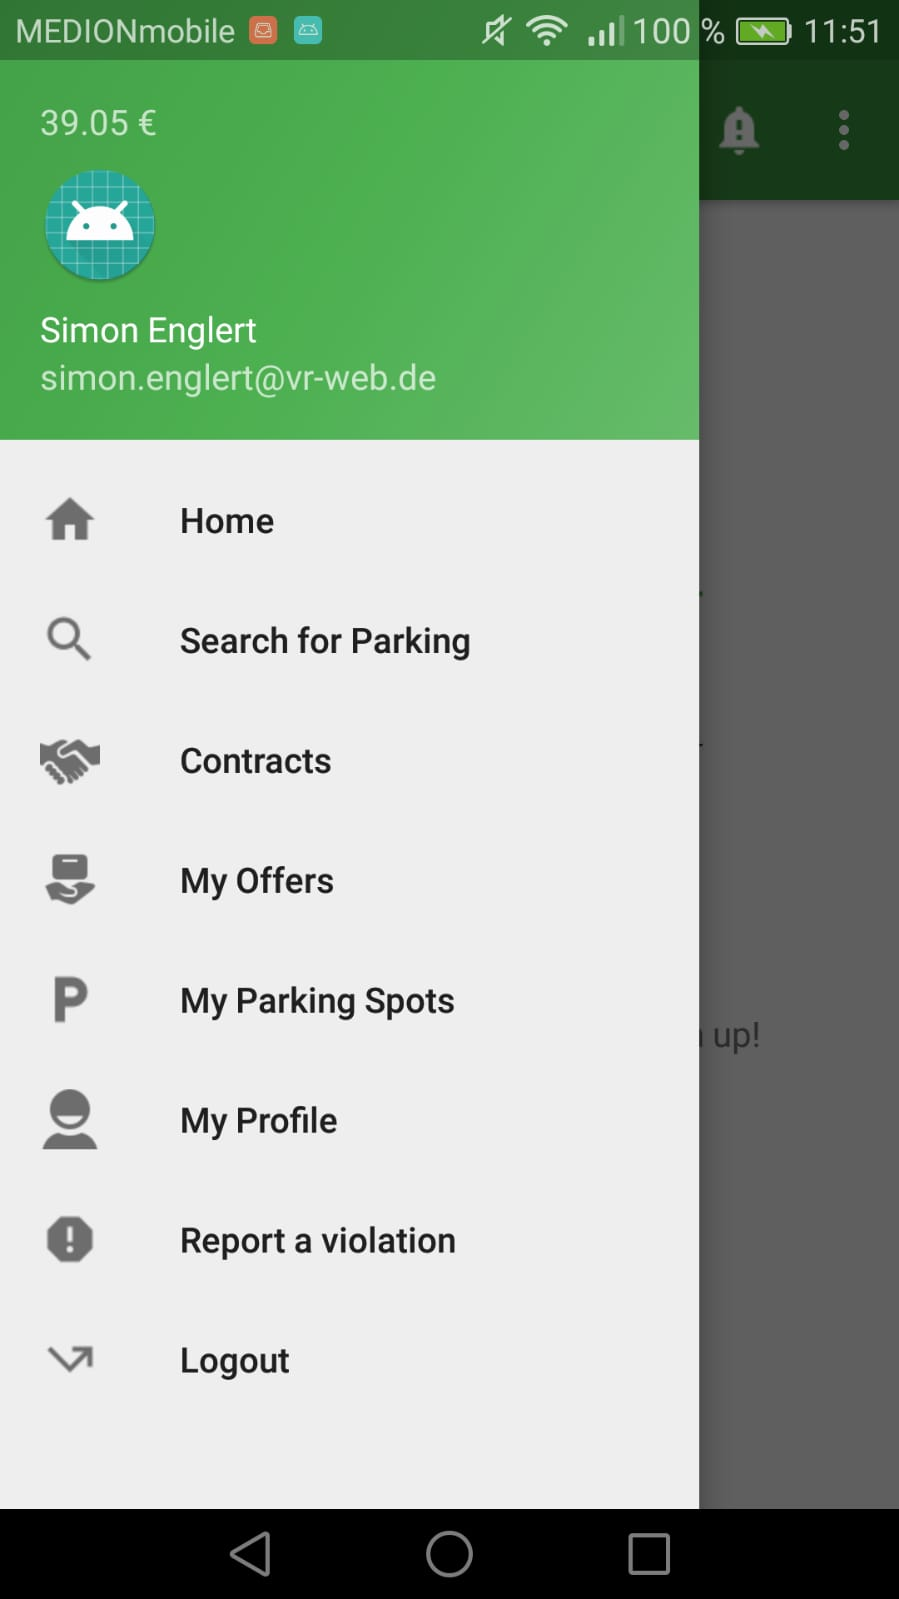
\includegraphics[height=11cm]{logos/screenshot-menu.png}
	\caption{A screenshot of the drawer menu of the prototype}
	\label{img:screenshot-menu}
\end{figure}

\begin{figure}
	\centering
	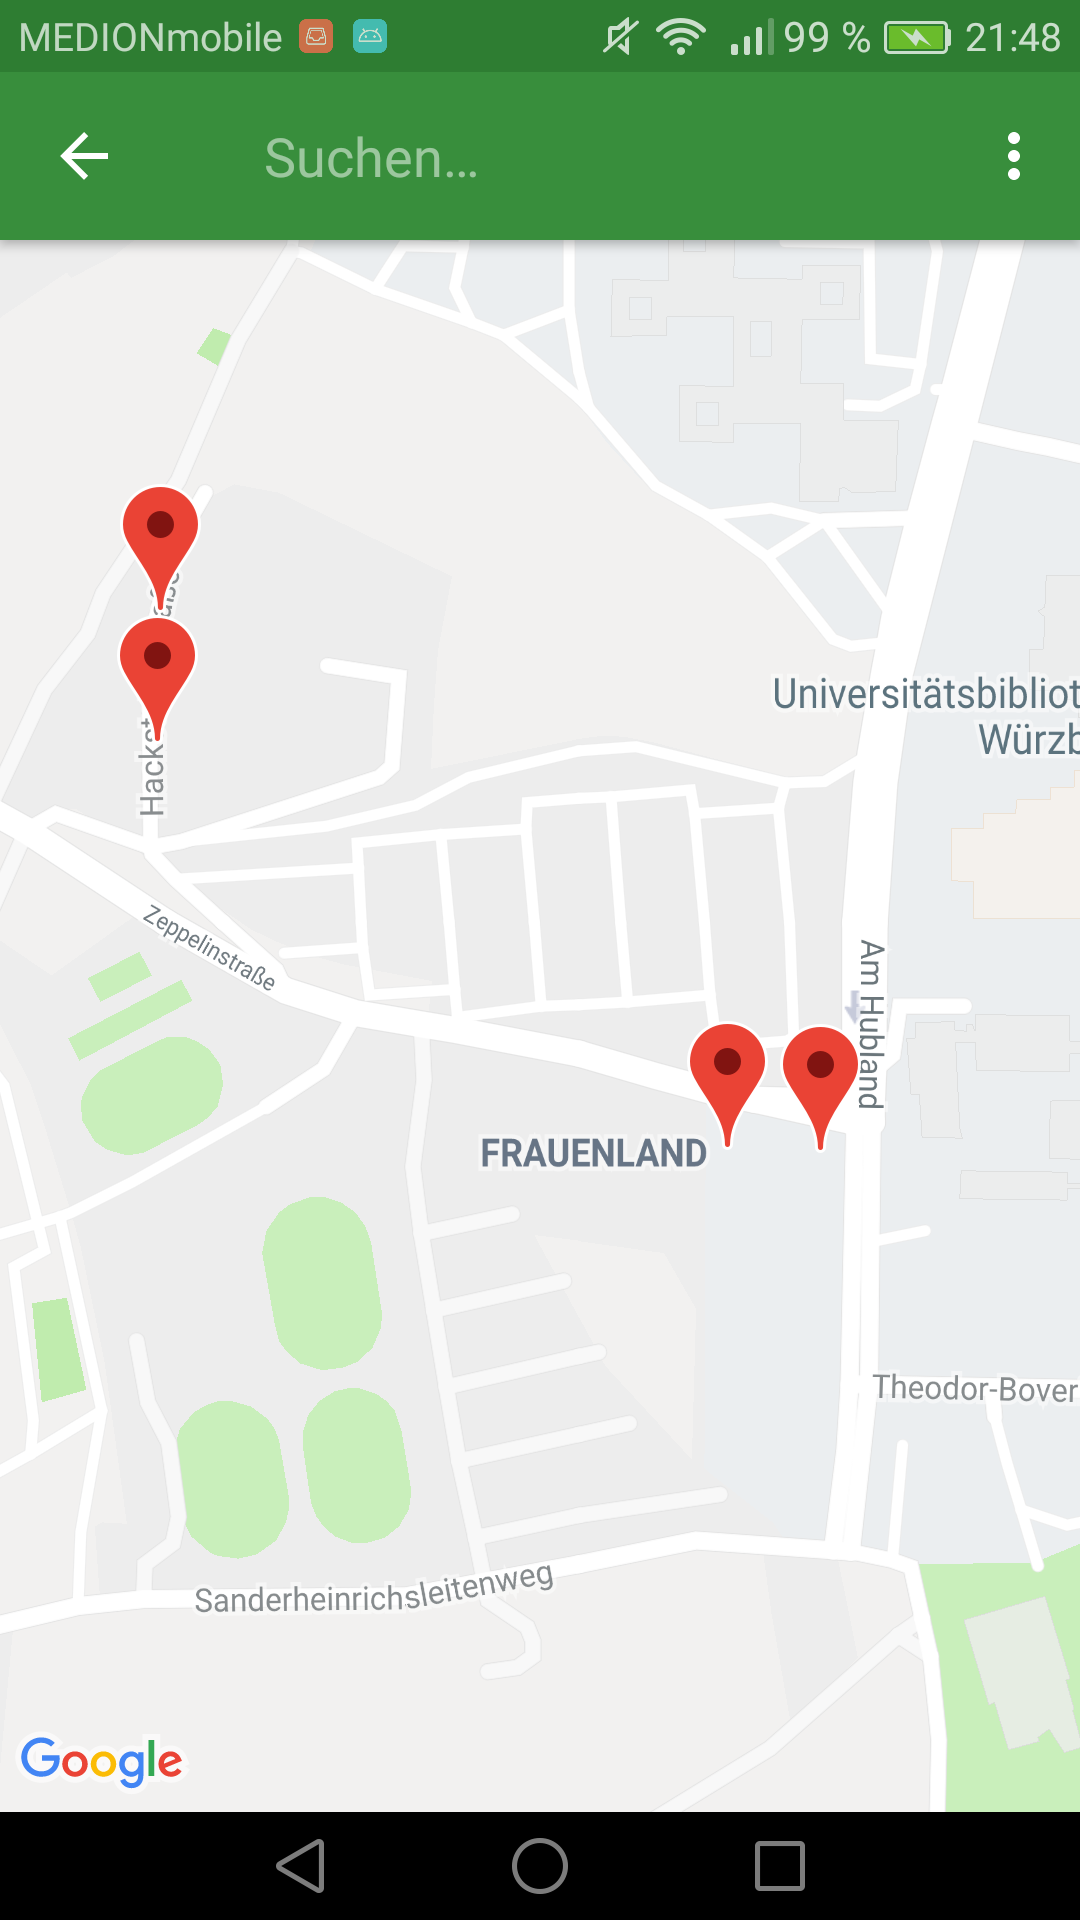
\includegraphics[height=11cm]{logos/screenshot-search.png}
	\caption{A screenshot of the parkingplace search feature of the prototype}
	\label{img:screenshot-search}
\end{figure}

\subparagraph{Instructions for use}
One has to adjust the static String BASE\_URL found in line 21 of NetworkUtilities.java in the package networking to the server address of the Java web service. The whole project can for example be imported into Android Studio and the app can be run on a connected android smartphone or an emulated device in Android Studio.

\section{Comments on the realization of the $SPS$}\label{sec:Comments on the realization}

\subparagraph{Creation of a basic user structure}
The problem of many shared parking systems mentioned in section x is that they could hardly generate any users at all. One of the reasons for this is probably that such a system must first overcome a certain barrier before it becomes attractive for users. Nobody registers with a system to lease parking spaces if there is no one renting them out. And no private user takes the trouble to insert a parking space that nobody will ever book. The pure C2C model is actually not really suited for the launch of such a system. However, businesses can help to overcome this barrier. Various buisenesses such as hotels, cinemas, doctors or supermarkets usually only need their parking spaces for a certain period of the day. If one has already contacted some of the above mentioned before launching the system and they decide to insert their parking spaces, the system already launches with a large supply of parking spaces. This supply can then also ensure that demand increases and the system further grows.

\subparagraph{Solution for adversaries not registered in the system}
In section x the problem has already been raised that it is not possible to punish parking offenders directly via the $SPS$ if they are not part of the system. However, there is also a solution that can be implemented when realizing the system.

Without the $SPS$, adversaries in private parking spaces can only be punished by requesting a towing service and having the parking space cleared. There are, however, two problems: On the one hand, all costs that the adversary has to pay are transferred to the towing service and cannot be used by the $SPS$ to pay for a replacement parking space or inspectors. On the other hand, it can happen that the adversary has already left the parking space when the towing service arrives and the caller has to cover the costs.

However, the situation that several towing services are competing with each other in larger cities can be taken advantage of. It should be possible to negotiate a deal with one of the towing services stating that all towing operations under the $SPS$ will be carried out by this service provider. In return, the service provider pays part of its extremely high towing fee back to the $SPS$, which can then be used to pay for the replacement parking space and the inspectors. In addition, service provider should not charge any costs in the event that the adversary has already left the car park. In return, every report, that contains a license plate which is not registered in the system, is forwarded directly to the towing service. In this way, both parties can benefit from the deal.